\documentclass[aspectratio=169, table]{beamer}
\usepackage[utf8]{inputenc}
\usepackage[T1]{fontenc}
\usepackage{graphicx}
\usepackage{fontspec} 
\usepackage{xcolor}
\usepackage{tcolorbox}
\usepackage{listings} % Add the listings package
\lstset{
  breaklines=true, % Enable line wrapping
  % ... (other style settings)
}
\setsansfont[
ItalicFont=fonts/TitilliumWeb-Italic.ttf,
BoldFont=fonts/TitilliumWeb-Bold.ttf,
BoldItalicFont=fonts/TitilliumWeb-BoldItalic.ttf,
]{TitilliumWeb-Regular.ttf}

% Custom CSS language definition
\lstdefinelanguage{CSS}{
    keywords={color, background, margin, padding, font-size, text-align, border},
    keywordstyle=\color{blue}\bfseries,
    ndkeywords={url},
    ndkeywordstyle=\color{orange}\bfseries,
    identifierstyle=\color{black},
    sensitive=false,
    comment=[l]{//},
    morecomment=[s]{/*}{*/},
    commentstyle=\color{gray}\ttfamily,
    stringstyle=\color{green}\ttfamily,
}

% Custom JavaScript language definition
\lstdefinelanguage{JavaScript}{
    keywords={function, var, let, const, if, else, for, while, return, true, false},
    keywordstyle=\color{blue}\bfseries,
    ndkeywords={class, export, boolean, throw, implements, import, this},
    ndkeywordstyle=\color{orange}\bfseries,
    identifierstyle=\color{black},
    sensitive=false,
    comment=[l]{//},
    morecomment=[s]{/*}{*/},
    commentstyle=\color{gray}\ttfamily,
    stringstyle=\color{green}\ttfamily,
}

\subtitle{IF140303 Web-based Application Development}
\title{\Huge {\textbf{03: \\JavaScript}}}
\date[Serial]{\scriptsize {PRU/SPMI/FR-BM-18/0222}}
\author[Pradita]{\small {\textbf{PRADITA UNIVERSITY}}}

\usetheme{Pradita} %To change Styles of the ppt

\begin{document}
\begin{frame}
    \titlepage
\end{frame}

\begin{frame}{Goals}
    \vskip-1cm
    \begin{itemize}
        \item To learn about JavaScript and its role in web development
        \item To understand how JavaScript is used to add interactivity and dynamic behavior to web pages
        \item To learn about JavaScript functions, variables, and control flow structures
        \item To apply JavaScript code to enhance the functionality of the currency converter web page from the previous session
    \end{itemize}
\end{frame}

\begin{frame}{Introduction to JavaScript}
    \vskip-0.5cm
    \begin{itemize}
        \item JavaScript is a high-level, interpreted scripting language primarily used for web development.
        \item It is often described as the "language of the web" as it allows developers to create interactive and dynamic web pages.
        \item JavaScript enables client-side scripting, meaning it runs directly in the web browser and can interact with the HTML and CSS of a web page.
        \item With JavaScript, you can respond to user actions, manipulate the DOM (Document Object Model), and perform asynchronous operations, such as fetching data from servers.
    \end{itemize}
\end{frame}

\begin{frame}[fragile] % Add the 'fragile' option here
    \frametitle{Basic JavaScript Syntax}
    \vskip0.5cm
    \begin{lstlisting}[language=JavaScript]
// JavaScript comment
function functionName(parameter) {
    // function body
    return result;
}

// Example
function addNumbers(a, b) {
    return a + b;
}
    \end{lstlisting}
\end{frame}

\begin{frame}{JavaScript Variables}
    \begin{tcolorbox}[standard jigsaw, opacityback=0, opacityframe=0, sharp corners, boxrule=0pt]
        \textbf{\textcolor{white}{In JavaScript, you can use variables to store data values. Some key points about variables:}}
        \begin{itemize}
            \item Variables are declared using the \texttt{var}, \texttt{let}, or \texttt{const} keyword.
            \item \texttt{var} was the traditional way to declare variables, but \texttt{let} and \texttt{const} are recommended in modern JavaScript.
            \item \texttt{let} allows reassigning the value of a variable, while \texttt{const} creates a read-only (constant) variable.
            \item Variables can store various data types, such as numbers, strings, arrays, objects, and more.
        \end{itemize}
    \end{tcolorbox}
\end{frame}

\begin{frame}{JavaScript Control Flow}
    \begin{tcolorbox}[standard jigsaw, opacityback=0, opacityframe=0, sharp corners, boxrule=0pt]
        \textbf{\textcolor{white}{Control flow structures in JavaScript allow you to make decisions and perform actions based on conditions. Common structures include:}}
        \begin{itemize}
            \item \texttt{if} statement: Executes a block of code if a specified condition is true.
            \item \texttt{else} statement: Executes a block of code if the \texttt{if} condition is false.
            \item \texttt{else if} statement: Checks additional conditions after the initial \texttt{if} condition.
            \item \texttt{switch} statement: Evaluates an expression and executes different code blocks based on its value.
            \item \texttt{for} loop: Repeats a block of code for a specified number of times.
            \item \texttt{while} loop: Repeats a block of code as long as a specified condition is true.
        \end{itemize}
    \end{tcolorbox}
\end{frame}

\begin{frame}[fragile]
    \frametitle{Javascript converter.js}
    \begin{itemize}
            \item \texttt Create file converter.js
            \item \texttt Add <script src="assets/js/converter.js"></script> to converter.html
	 \item \texttt Register an account in https://app.freecurrencyapi.com/
	 \item \texttt Copy the url adding it to url variable in tutorial
            \item \texttt Function for Reverse Button (Next Pages)
            \item \texttt Function for Convert Button (Next Pages)
        \end{itemize}
\end{frame}

\begin{frame}[fragile]
    \frametitle{Javascript Reverse Button}
    \begin{lstlisting}[language=JavaScript]
const reverseButton = document.getElementById("reverse");
reverseButton.addEventListener("click", function () {
  const fromSelect = document.getElementById("from");
  const toSelect = document.getElementById("to");
  const temp = fromSelect.value;
  fromSelect.value = toSelect.value;
  toSelect.value = temp;
});
    \end{lstlisting}
\end{frame}

\begin{frame}[fragile]
    \frametitle{Convert Button - Part 1}
    \begin{lstlisting}[language=JavaScript]
const convertButton = document.getElementById("convert");
convertButton.addEventListener("click", async function () {
  const fromSelect = document.getElementById("from");
  const toSelect = document.getElementById("to");
  const url = "https://api.freecurrencyapi.com/v1/latest?apikey=fca_live_iq1WvbaON67X9adHTaJiqEszDhP6jtDz7IouUbWv&currencies=" + toSelect.value + "&base_currency=" + fromSelect.value;
  const options = {
    method: "GET",
  };
    \end{lstlisting}
\end{frame}

\begin{frame}[fragile]
    \frametitle{Convert Button - Part 2}
    \begin{lstlisting}[language=JavaScript]
 try {
    const response = await fetch(url, options);
    const result = await response.text();
    const amount = document.getElementById("amount").value;
    const rate = result.split(":")[2].split("}")[0];
    const converted = (amount * rate).toLocaleString(undefined, {
      minimumFractionDigits: 2,
      maximumFractionDigits: 2,
    });
    \end{lstlisting}
\end{frame}

\begin{frame}[fragile]
    \frametitle{Convert Button - Part 3}
    \begin{lstlisting}[language=JavaScript]
   let fromCurrencySymbol;
    if (fromSelect.value === "IDR") {
      fromCurrencySymbol = "Rp. ";
    } else if (fromSelect.value === "USD") {
      fromCurrencySymbol = "$ ";
    } else if (fromSelect.value === "EUR") {
      fromCurrencySymbol = "€ ";
    } else if (fromSelect.value === "GBP") {
      fromCurrencySymbol = "£ ";
    }
    \end{lstlisting}
\end{frame}

\begin{frame}[fragile]
    \frametitle{Convert Button - Part 4}
    \begin{lstlisting}[language=JavaScript]
   let toCurrencySymbol;
    if (toSelect.value === "IDR") {
      toCurrencySymbol = "Rp. ";
    } else if (toSelect.value === "USD") {
      toCurrencySymbol = "$ ";
    } else if (toSelect.value === "EUR") {
      toCurrencySymbol = "€ ";
    } else if (toSelect.value === "GBP") {
      toCurrencySymbol = "£ ";
    }
    \end{lstlisting}
\end{frame}

\begin{frame}[fragile]
    \frametitle{Convert Button - Part 5}
    \begin{lstlisting}[language=JavaScript]
    const fromResult = document.getElementById("from-result");
    const fromCurrency = document.getElementById("from-currency");
    const toResult = document.getElementById("to-result");
    fromResult.textContent = fromCurrencySymbol + amount;
    fromCurrency.textContent = fromSelect.value;
    toResult.textContent = toCurrencySymbol + converted;
    document.getElementById("to-currency").textContent
    = toSelect.value;
    \end{lstlisting}
\end{frame}

\begin{frame}[fragile]
    \frametitle{Convert Button - Part 6}
    \begin{lstlisting}[language=JavaScript]
    const exchangeRateLabel = document.getElementById("exchange-rate");
    const formattedRate = parseFloat(rate).toFixed(2);
    const exchangeRateText = `1 ${fromSelect.value} = ${formattedRate} ${toSelect.value}`;
    exchangeRateLabel.textContent = exchangeRateText;
  } catch (error) {
    console.error(error);
  }
});
    \end{lstlisting}
\end{frame}

\begin{frame3}
    \vskip1cm
    \begin{tcolorbox}[standard jigsaw, opacityback=0, opacityframe=0, sharp corners, boxrule=0pt]
        \begin{columns}[T] %T for Top, C for Center, B for Bottom
            \begin{column}{0.5\textwidth}
                \textbf{\textcolor{white}{JavaScript adds interactivity to web pages, allowing users to interact with and modify the content dynamically. By using functions, variables, and control flow structures, you can create responsive web applications that adapt to user actions.}}
            \end{column}
            \begin{column}{0.5\textwidth}
                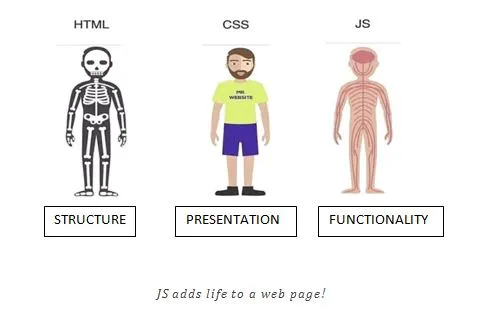
\includegraphics[width=1\textwidth]{classFiles/js_interactivity.png}
            \end{column}
        \end{columns}
    \end{tcolorbox}
\end{frame3}

\begin{frame4}
    \frametitle{Thank You}
\end{frame4}

\end{document}
